\documentclass[aps,reprint,superscriptaddress,10pt]{revtex4-2}
\usepackage{kotex}
\usepackage[HWP]{dhucs-interword}
\usepackage[dvips]{color}
\usepackage{graphicx}
\usepackage{bm}
\usepackage{amsmath}
\usepackage{tikz}
\usepackage{mhchem}
\usepackage{booktabs}
\usepackage{multirow}
\usepackage{array}
\usepackage{tikz}

\begin{document}
\title{응집물질물리실험 예비보고서 \\
\small 실험주제 : Hall Effect}

\author{HuiJae-Lee}

\affiliation{Physics Department, Inha University}
\email{hjlee6674@inha.edu}

\date{\today}


\begin{abstract}
이번 실험은 임계온도 미만에서 초전도체가 가지는 반자성과 완전 도체 성질을 확인하고
히스테리시스 곡선을 통해 물질의 자화 현상을 이해하며 Seebeck effect를 공부하는 것을
목표로 한다.
\end{abstract}
 
 \maketitle
 
\section[Introduction]{Introduction}
초전도체는 0인 전기 저항을 가진다는 특성에 의해 각종 분야에서 이용되고 있다.
주로 강한 전류를 필요로 하는 핵융합, 입자가속기 등의 첨단 과학 분야에서 그 성질을
발휘하고 있으며 MRI, 자기부상열차와 같이 일상과 밀접하게 응용되고 있기도 하다.
Hysteresis는 자성체가 자화되고 풀릴 때 발생하는 일반적인 현상으로 변압기의 전력 손실을
파악할 때 주요한 현상 중 하나이다. Seebeck effect는 온도차를 이용해 전위차를 만들어내는
현상으로 열적 현상과 전기적 현상을 연결하는 열전대(thermoelectric) 현상의 대표적인
예시이다. 열적 손실로 인해 버려지는 에너지를 이용하는데 응용되고 있으며 같은 열전대 현상인
Peltier effect는 전기 에너지로 온도차를 발생시켜 전자기기를 냉각하는 장치에 이용되는 등
다양한 방면에서 이용되고 연구되는 중이다.
\section{Experiment}

\subsection{Theory}
\subsubsection{Superconductor}
초전도성은 시료를 저온 영역으로 냉각시킬 때 전기 비저항이 0으로 떨어지는 성질이다.
비저항이 0이 되므로 초전도체는 저항이 없는 완전 도체의 성질을 가지게 된다.
초전도체가 가지는 특이한 성질 중 하나는 반자성이다. 초전도체는 임계온도보다 냉각되면
내부 자기장이 0이 되어 외부 자기장을 밀어낸다. 이 효과를 마이스너 효과라 부른다. 
이런 초전도성은 충분히 강한 외부 자기장에 의해 깨질 수 있고 이 자기장의 임계값은
물질에 따라 다르다. \\
제 1형 초전도체는 온도와 외부 자기장의 크기에 따라 초전도성이 명확하게 보여지고 사라지는
물질이다. 제 1형 초전도체는 보통 상태와 초전도 상태만을 가진다(FIG.~\ref{fig:1}). 
\begin{figure}[htbp]
  \centering
  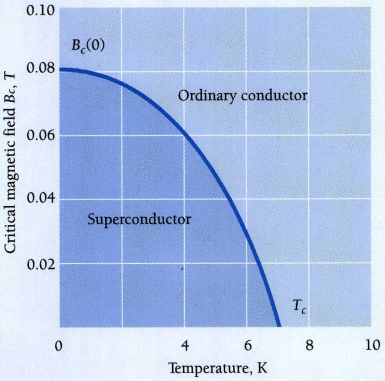
\includegraphics[scale = 0.5]{1.png}
  \caption{제 1형 초전도체 중 하나인 납이 초전도성을 유지할 수 있는 영역을 표시한 좌표평면}
  \label{fig:1}
\end{figure}

제 2형 초전도체는 제 1형 초전도체와 다르게 보통 상태와 초전도 상태의 혼합상태를 가질 수 있다.
혼합상태에서 제 2형 초전도체는 내부에 자기 선속을 가지고 있으면서 
초전도성을 유지한다(FIG.~\ref{fig:2}).

\begin{figure}[htbp]
  \centering
  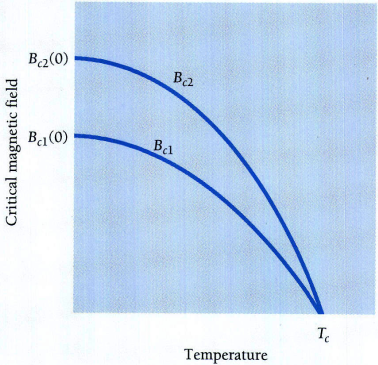
\includegraphics[scale = 0.5]{2.png}
  \caption{제 2형 초전도체가 온도와 외부 자기장에 따라 가질 수 있는 상태를 나타낸 그림}
  \label{fig:2}
\end{figure}


\subsubsection{Magnetization}
일반적으로 물체는 그 내부의 자기 모멘트가 무작위하게 배열되어 있어 서로 상쇄되기 
때문에 거시적으로 자성을 가지지 않는 것 처럼 보인다. 외부에서 이런 물체에 자기장을
걸어주면 무작위하게 배열되어 있던 자기 모멘트가 자기장을 따라 일정한 방향으로 배열되어
자성의 띄게 되는데 이러한 현상을 자화라 부른다. 미시적으로 본 자유원자의 자기 모멘트는
전자의 스핀, 핵에 대한 궤도 각운동량, 외부 자기장에 의한 궤도 각운동량의 영향을 받는다.
자기화를 나타내는 벡터량인 자화밀도 $\vec{M}$은 단위 부피 속에 포함된 자기 쌍극자
모멘트로 정의된다. 대부분의 물질의 자화밀도는 자기장이 너무 강하지 않은 한 자기장에 비례한다.
따라서 자기장과 자화밀도의 비인 자기 감수율 $\chi$를 다음과 같이 정의할 수 있다.
\begin{align}
  \chi = \frac{\mu_0M}{B}
\end{align}
$M,\,B$는 각각 자화밀도의 크기, 자기장의 크기이다. 이 자기 감수율이 음수인 물질을
반자성체, 양수인 물질을 상자성체라 부른다.


\subsubsection{Hysteresis}
물체를 강하게 자화시켜 모든 자기 쌍극자가 같은 방향으로 정렬되면 물체의 자화상태는 
포화되었다고 말한다. 이 상태에서는 자기장을 더 강하게 걸어주더라도 자화밀도 $\vec{M}$이
더 커지지 않는다. 이제 자기장을 점점 줄이면 물체의 자화가 천천히 풀린다. 하지만
물체 내 자기 쌍극자가 서로 영향을 주고 받으므로 자화밀도는 자기장에 따라 증가한대로
감소하지 않는다. 즉, 처음에 자화되어있지 않았던 물체($B=0,\,M=0$)를 포화된 자화상태로 만든 뒤, 
자기장을 제거하더라도 물체의 자화는 완전히 풀리지 않는다($B=0,\,M\neq0$). 이제 자기장을
자화된 방향의 반대로 걸어주면 물체의 자화가 풀렸다가 외부 자기장을 따라 다시 자화된다.
이 현상을 그래프로 표현하였을 때 나타나는 곡선을 Hysteresis 곡선이라 
부른다(FIG.~\ref{fig:hy}).
\begin{figure}[htbp]
  \centering
  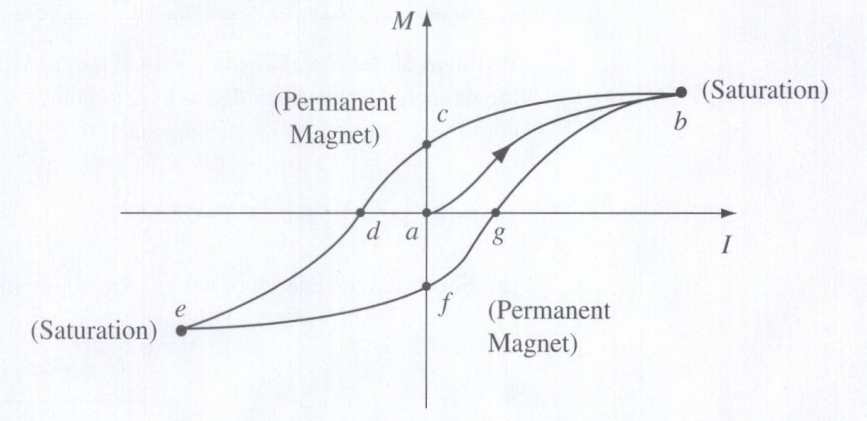
\includegraphics[scale = 0.28]{hy.png}
  \caption{자기장을 생성하는 전류의 크기를 $x$축으로 하고
  물체의 자화밀도를 $y$축으로 한 Hysteresis 곡선}
  \label{fig:hy}
\end{figure}






\subsubsection{Seebeck effect}
Seebeck effect는 온도차로 인해 전위차가 유도되는 현상으로 온도차로 인해 전자가 가지는
에너지가 달라져 발생한다. FIG.~\ref{fig:see}와 같이 다른 도체로 구성된 회로를 생각하자.
$a$와 $b$는 직렬로 연결되어 있고 열적 평형 상태에 있다. 만약 연결부인 $A$와 $B$가 서로
다른 온도 $T_1$, $T_2$($T_1>T_2$)로 유지된다면 열린 회로의 기전력 $V$가 $C$와 $D$ 사이에 다음과
같이 유도된다.
\begin{align}
  V = \alpha(T_1-T_2)
\end{align}
$\alpha$는 Seebeck coefficient라고 불린다. 작은 온도차에서 이 관계는 선형적이다.
\begin{figure}[htbp]
  \centering
  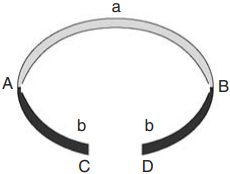
\includegraphics[scale = 0.6]{seebeck.png}
  \caption{Seebeck effect를 설명하기 위한 열린 회로}
  \label{fig:see}
\end{figure}








\subsection{Experimental Methods}
\subsubsection{Superconductivity}
\begin{itemize}
  \item[1. ] 초전도체의 반자성 성질을 확인하기 위해 네오디뮴 자석, 초전도체 혼합물, 
  Meissner-Ochsenfeld effect experiment kit을 준비한다.
  \item[2. ]
  Meissner-Ochsenfeld effect experiment kit 위에 초전도체 혼합물을 올려놓고 
  액화질소를 이용해 초전도체를 냉각시킨다.
  \item[3. ]
  냉각된 초전도체 위에 자석을 올려놓고 자석이 공중에 뜨는 것을 통해 초전도체의 반자성
  성질을 확인한다.
  \item[4. ] 초전도체의 완전 도체 성질을 확인하기 위해 초전도체 실험용 키트 및 샘플과
  메스 어댑터, Sensor-Cassy2를 준비한다.
  \item[5. ] 메스 어댑터, Sensor-Cassy2와 컴퓨터를 연결한다. 
  \item[6. ] Cassy Lab software를 열고 프로그램을 실행시킨다.
  \item[7. ] 초전도체를 액화질소로 냉각시켜가며 온도에 따른 전압을 측정한다.
  \item[8. ] -180$^\circ$C로 냉각된 초전도체를 해동시키며 온도에 따른 전압을 측정한다.  
\end{itemize}
\subsubsection{Hysteresis of Transformer Core}
\begin{itemize}
  \item[1. ] 컴퓨터, 함수발생기, 코일 및 자성체, 연결선을 준비한다.
  \item[2. ] 컴퓨터를 키고 실험용 프로그램을 실행시킨다.
  \item[3. ] 함수발생기 및 각 키트를 연결선으로 연결하고 이를 다시 컴퓨터에 연결하여
  연결 상태를 확인한다.
  \item[4. ] 함수발생기의 입력 파형, 주파수, 전압 진폭을 바꿔가며 히스테리시스 곡선의
  형태를 측정하고 데이터를 저장한다.
  \item[5. ] 입력 파형(사인파, 삼각파, 사각파), 주파수(0.1 Hz, 1 Hz, 2 Hz), 
  전압 진폭(4V, 7V, 10V)을 바꿔가며 결과를 측정한다. 각 조건을 바꿀 때 마다
  자성체의 방향을 변경하여 자화된 상태의 영향을 덜 받도록 한다.
  \item[6. ] 얻은 데이터를 통해 결과를 분석한다.
\end{itemize}
\subsubsection{Calibrating of Thermocouple}
\begin{itemize}
  \item[1. ] 금속 도선, 온도계, 전압계, 핫플레이트, 얼음, 물, 비커를 준비한다.
  \item[2. ] 두 비커에 각각 물, 얼음을 채우고 온도계를 설치한다.
  \item[3. ] 물이 담긴 비커는 핫플레이트 위에 놓는다.
  \item[4. ] 금속 도선의 접합부를 두 비커 안에 두고 전압계에 연결한다.
  \item[5. ] 온도계의 눈금과 전압계의 전압을 기록한다.   
\end{itemize}

\nocite{*} 
\bibliography{ref}



%\begin{thebibliography}{9}
%\end{thebibliography}

\vfill
\end{document}